% !TEX root = main.tex
\documentclass[11pt,a4paper]{article}

% --- PACHETE NECESARE ---
\usepackage[T1]{fontenc}      % Corectare afisare diacritice
\usepackage[romanian]{babel} 
\usepackage[utf8]{inputenc}
\usepackage{csquotes}
\usepackage{indentfirst}
\usepackage{graphicx}
\usepackage{float} 
\usepackage{hyperref}
% MINTED necesita Python instalat + pygments.
% Compilare: pdflatex -shell-escape proiect.tex
\usepackage{minted} 
\usepackage{xcolor}
\usepackage{geometry}
\usepackage{tocloft}
\usepackage{cite}

% --- CONFIGURARE PAGINA ---
\geometry{top=2.5cm, bottom=2.5cm, left=2.5cm, right=2.5cm}
\linespread{1.1}
\hypersetup{colorlinks, citecolor=black, filecolor=black, linkcolor=black, urlcolor=black}
\renewcommand{\cftsecleader}{\cftdotfill{\cftdotsep}}

% --- SURSA BIBLIOGRAFICA ---
\begin{filecontents}{refs.bib}
@misc{catmullrom,
    author = {{Wikipedia Contributors}},
    title = {Catmull–Rom spline},
    year = {2026},
    publisher = {Wikipedia, The Free Encyclopedia},
    url = {https://en.wikipedia.org/wiki/Catmull%E2%80%93Rom_spline},
    note = {Accesat la 10 Ianuarie 2026}
}

@manual{lab7,
    author = {Adrian Sabou},
    title = {Laborator 7: Iluminare - Modelul Phong},
    organization = {Universitatea Tehnica din Cluj-Napoca},
    note = {Prelucrare Grafica},
    year = {2025}
}

@manual{lab9,
    author = {Adrian Sabou},
    title = {Laborator 9: Tehnici de randare a umbrelor (Shadow Mapping)},
    organization = {Universitatea Tehnica din Cluj-Napoca},
    note = {Prelucrare Grafica},
    year = {2025}
}

@misc{model_nanosuit,
    author = {{Crytek}},
    title = {Nanosuit 3D Model},
    year = {2011},
    url = {https://free3d.com/3d-model/crysis-2-nanosuit-2-97837.html},
}
@misc{model_mario,
    author = {{Nintendo}},
    title = {Mario 3D Model},
    year = {2025},
    url = {https://sketchfab.com/3d-models/mario-ds-fbx-552baccb1ef74a799fb7440fdc5fd69d#download},
}
@misc{model_creeper,
    author = {{Mojang Studios}},
    title = {Creeper 3D Model},
    year = {2009},
    url = {https://sketchfab.com/3d-models/minecraft-creeper-c986450b4d884c2c94c0d3168671c543#download},
}
@misc{model_zombie,
    author = {{Mojang Studios}},
    title = {Zombie 3D Model},
    year = {2009},
    url = {https://sketchfab.com/3d-models/minecraft-zombie-45037ec52b6a4444a0981f916d0dbd43#download},
}
@misc{model_diamond,
    author = {{Mojang Studios}},
    title = {Diamond Ore Texture},
    year = {2010},
    url = {https://texture-packs.com/resourcepack/default-pack/},
}
@misc{tex_ground,
    author = {{Mojang Studios}},
    title = {Grass Texture},
    year = {2009},
    url = {https://texture-packs.com/resourcepack/default-pack/},
}
@misc{tex_vegetation,
    author = {{Tech Monkey Bussines}},
    title = {Vegetation Billboard Texture},
    year = {2026},
    url = {https://www.techmonkeybusiness.com/galleries/Texture_Galleries/Billboard_Trees/},
}
@misc{tex_skybox,
    author = {{Mojang Studios}},
    title = {Minecraft Skybox Texture},
    year = {2011},
    url = {https://texture-packs.com/resourcepack/default-pack/},
}
\end{filecontents}


\begin{document}

% Rezolva problema avertismentelor "page 1 duplicate"
\pagenumbering{Alph}

% ===================================================================
% PAGINA DE INCEPUT
% ===================================================================
\begin{titlepage}
    \centering
    \vspace*{2cm}
    {\Huge \textbf{Universitatea Tehnica din Cluj-Napoca}} \par
    \vspace{1cm}
    {\Large Facultatea de Automatica si Calculatoare} \par
    \vspace{3cm}
    \rule{\linewidth}{0.5mm} \par
    \vspace{0.4cm}
    {\huge \textbf{Documentatie Proiect: Scena {3D} Interactivă}} \par
    \vspace{0.4cm}
    \large Sisteme de Prelucrare Grafica (SPG) \par
    \vspace{0.4cm}
    \rule{\linewidth}{0.5mm} \par
    \vspace{4cm}
    \begin{minipage}{0.4\textwidth}
        \begin{flushleft} \large
            \emph{Autor:}\\
            Stolniceanu Iustin-Pavel
        \end{flushleft}
    \end{minipage}
    \begin{minipage}{0.4\textwidth}
        \begin{flushright} \large
            \emph{Profesor coordonator:} \\
            Constantin Nandra
        \end{flushright}
    \end{minipage}
    \vfill
    {\large Ianuarie 2026}
\end{titlepage}

% ===================================================================
% 1. CUPRINS
% ===================================================================
\newpage
\tableofcontents
\newpage

% Reseteaza numerotarea pentru continut
\cleardoublepage
\pagenumbering{arabic}

% ===================================================================
% 2. PREZENTAREA TEMEI
% ===================================================================
\section{Prezentarea temei}
Acest proiect are ca scop realizarea unei scene 3D fotorealiste si interactive, dezvoltata in C++ utilizand API-ul grafic OpenGL 4.1. Arhitectura aplicatiei se bazeaza pe o suita de biblioteci specializate: \textbf{GLFW} pentru managementul ferestrei si a input-ului, \textbf{GLEW} pentru gestionarea extensiilor OpenGL si \textbf{GLM} (OpenGL Mathematics) pentru operatii vectoriale si matriceale.

Proiectul demonstreaza stapanirea conceptelor fundamentale din grafica computerizata, de la managementul resurselor (modele, texturi, shadere) la implementarea unor tehnici avansate precum:
\begin{itemize}
    \item Iluminare complexa bazata pe modelul Phong, incluzand surse de lumina multiple (directionala, punctiforma si spotlight).
    \item Randarea umbrelor dinamice pentru lumina directionala prin tehnica \textit{Shadow Mapping}.
    \item Optimizarea randarii pentru scene complexe, folosind tehnica \textit{billboarding} pentru vegetatie.
    \item Managementul camerei la persoana intai, cu detectie de coliziuni si o traiectorie cinematica pre-calculata (Catmull-Rom spline).
    \item Efecte de post-procesare simple, precum ceata (fog).
\end{itemize}

Obiectivul principal a fost crearea unui mediu virtual populat (o padure generata procedural), care sa permita explorarea libera si interactiunea cu diverse efecte dinamice, demonstrand o intelegere practica a pipeline-ului grafic modern.

% ===================================================================
% 3. SCENARIUL
% ===================================================================
\section{Scenariul}
\subsection{Descrierea scenei si a obiectelor}
Scena este compusa dintr-un teren vast, populat cu vegetatie si diverse obiecte 3D importate:
\begin{itemize}
    \item \textbf{Terenul:} Un plan texturat extins pentru a simula solul \cite{tex_ground}.
    \item \textbf{Vegetatia:} O padure compusa din peste 200 de copaci generati dinamic, folosind texturi de tip billboard \cite{tex_vegetation}.
    \item \textbf{Obiecte:} Nanosuit \cite{model_nanosuit}, Mario \cite{model_mario}, Creeper \cite{model_creeper}, Zombie \cite{model_zombie} si minereuri de diamant \cite{model_diamond}.
    \item \textbf{Skybox:} Un cubemap care ofera context vizual cerului, utilizand o textura dintr-un pachet de resurse Minecraft \cite{tex_skybox}.
\end{itemize}

% Imagini (Placeholders)
\begin{figure}[H]
    \centering
    % Daca ai imaginea, sterge % de la inceputul liniei urmatoare
    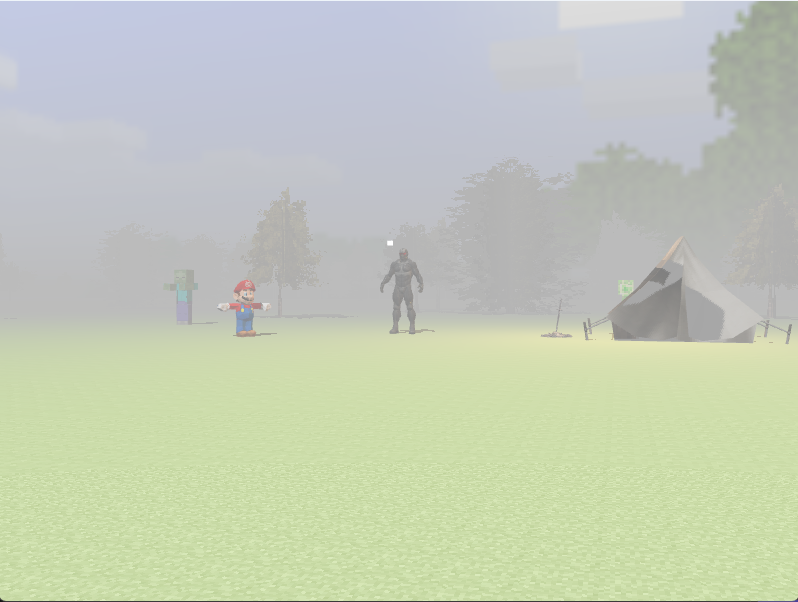
\includegraphics[width=0.7\textwidth]{resources/global_illumination.png}
    \caption{Vizualizarea scenei in conditii de iluminare globala (zi).}
\end{figure}

\begin{figure}[H]
    \centering
    % Daca ai imaginea, sterge % de la inceputul liniei urmatoare
     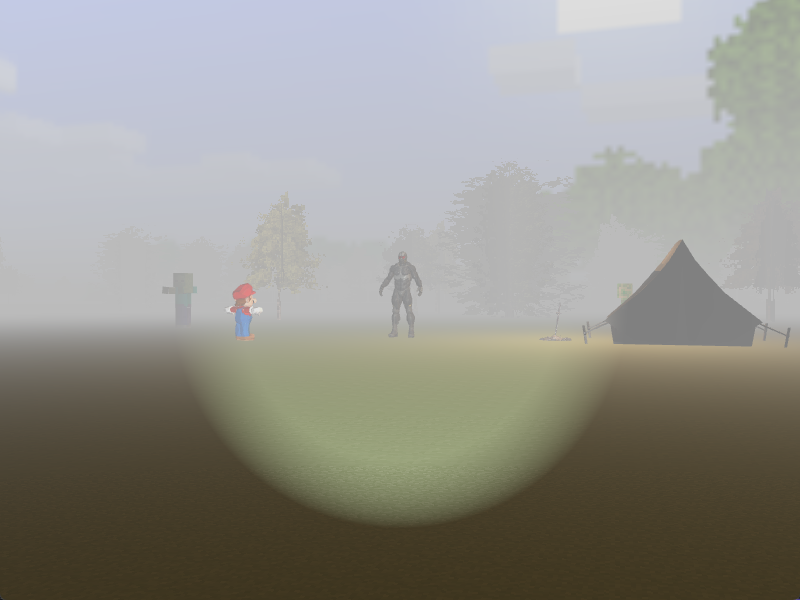
\includegraphics[width=0.7\textwidth]{resources/spotlight.png}
    \caption{Vizualizarea scenei cu lanterna (spotlight) activata pe timp de noapte.}
\end{figure}

\subsection{Functionalitati}
\begin{itemize}
    \item \textbf{Controlul Camerei:} Deplasare WASD si orientare prin mouse.
    \item \textbf{Iluminare Interactiva:} Comutare lanterna (tasta F).
    \item \textbf{Animatie Cinematica:} Traiectorie fluida bazata pe o curba spline \cite{catmullrom}.
    \item \textbf{Moduri de Vizualizare:} Solid, wireframe si polygonal points.
\end{itemize}

% ===================================================================
% 4. DETALII DE IMPLEMENTARE
% ===================================================================
\section{Detalii de implementare}

\subsection{Functii si algoritmi}
In aceasta sectiune sunt detaliate provocarile tehnice intampinate si solutiile algoritmice implementate pentru a asigura atat realismul vizual, cat si performanta necesara unei executii in timp real.

\subsubsection{1. Randarea vegetatiei: Tehnica Billboarding}
\textbf{Problema:} Crearea unei paduri dense (peste 200 de copaci) folosind modele 3D High-Poly ar fi dus la o scadere drastica a numarului de cadre pe secunda (FPS).

\textbf{Rezolvarea mea:} Am utilizat tehnica \textit{Static Cross-Quads}. Fiecare copac este reprezentat prin 3 planuri texturate care se intersecteaza la un unghi de 60°. Aceasta structura ofera iluzia de volum din orice unghi de vizualizare orizontal, utilizand doar 12 vertexuri.

\subsubsection{2. Detectia coliziunilor: Algoritmul AABB}
\textbf{Problema:} Navigarea intr-o scena populata necesita un sistem care sa impiedice camera sa treaca prin obiecte solide.

\textbf{Rezolvarea mea:} Am implementat volume de coliziune de tip \textit{Axis-Aligned Bounding Box} (AABB). Verificarea coliziunii se reduce la o serie de comparatii intre coordonatele camerei si limitele cutiei, rezultand intr-o complexitate de $O(1)$.

\subsubsection{3. Animatia camerei: Catmull-Rom Spline}
\textbf{Problema:} Definirea unei traiectorii automate fluide pentru cameră, care să treacă prin puncte de interes predefinite în scenă.

\textbf{Rezolvarea mea:} Am implementat o traiectorie fluidă bazată pe curba \textit{Catmull-Rom Spline} \cite{catmullrom}. Această tehnică este ideală pentru animații cinematice deoarece garantează că traiectoria va trece exact prin punctele de control specificate, generând o mișcare naturală și fără discontinuități.

Curba este definită parametric, calculând un punct \textbf{P(t)} pentru un segment determinat de patru puncte de control consecutive: \textbf{P0}, \textbf{P1}, \textbf{P2} și \textbf{P3}. Segmentul de curbă efectiv este desenat între \textbf{P1} și \textbf{P2}, în timp ce \textbf{P0} și \textbf{P3} sunt utilizate pentru a calcula tangenetele la capetele segmentului, asigurând astfel continuitatea C1 între segmente adiacente.

Formula matematică pentru un punct pe curbă este:
$P(t) = 0.5 \times ((2 \cdot P1) + (-P0 + P2) \cdot t + (2 \cdot P0 - 5 \cdot P1 + 4 \cdot P2 - P3) \cdot t^2 + (-P0 + 3 \cdot P1 - 3 \cdot P2 + P3) \cdot t^3)$

Unde `t` este un parametru care variază de la 0 la 1 și controlează poziția de-a lungul segmentului de curbă între \textbf{P1} și \textbf{P2}.

În implementarea mea, am definit un set de puncte de control (vectori `glm::vec3`) în scenă. Funcția `getSplinePoint` primește ca intrare timpul global al animației `t` și lista de puncte de control.

\begin{enumerate}
    \item \textbf{Identificarea segmentului curent:} Timpul global `t` este normalizat pentru a determina indexul primului punct de control al segmentului curent (\textbf{p1}). Celelalte puncte (\textbf{p0}, \textbf{p2}, \textbf{p3}) sunt calculate relativ la \textbf{p1}, asigurând continuitatea la capetele listei de puncte (traiectorie în buclă).
    
    \item \textbf{Calcularea parametrului local:} Partea fracționară a lui `t` devine parametrul local de interpolare pe segmentul curent.
    
    \item \textbf{Interpolarea:} Se aplică formula Catmull-Rom pentru a calcula coordonatele 3D exacte ale camerei pentru acel moment în timp. Poziția rezultată este apoi folosită pentru a actualiza matricea de vizualizare a camerei, creând iluzia unei mișcări continue și line.
\end{enumerate}

\begin{minted}[frame=lines, framesep=2mm, fontsize=\small]{cpp}
glm::vec3 getSplinePoint(float t, const std::vector<glm::vec3>& controlPoints) {
    int p0, p1, p2, p3;
    
    // Asigura o traiectorie in bucla (closed loop)
    p1 = (int)t % controlPoints.size();
    p2 = (p1 + 1) % controlPoints.size();
    p3 = (p2 + 1) % controlPoints.size();
    // Punctul anterior lui p1
    p0 = (p1 - 1 + controlPoints.size()) % controlPoints.size();

    // Parametrul local `t` intre p1 si p2
    float local_t = t - (int)t;

    // Formula Catmull-Rom
    float t2 = local_t * local_t;
    float t3 = t2 * local_t;

    glm::vec3 point = 0.5f * (
        (2.0f * controlPoints[p1]) +
        (-controlPoints[p0] + controlPoints[p2]) * local_t +
        (2.0f * controlPoints[p0] - 5.0f * controlPoints[p1] + 4.0f * controlPoints[p2] - controlPoints[p3]) * t2 +
        (-controlPoints[p0] + 3.0f * controlPoints[p1] - 3.0f * controlPoints[p2] + controlPoints[p3]) * t3
    );

    return point;
}
\end{minted}

\subsection{Modelul grafic}
Randarea scenei se bazeaza pe pipeline-ul programabil OpenGL (GLSL 4.10), orchestrat printr-o serie de programe de tip shader pentru a obtine efecte vizuale complexe.

\subsubsection{1. Umbre dinamice: Shadow Mapping}
Implementarea umbrelor pentru lumina directională (soarele) respecta algoritmul standard de \textit{Shadow Mapping} \cite{lab9}. Procesul este impartit in doua etape distincte (pass-uri) pentru fiecare cadru randat:

\begin{enumerate}
    \item \textbf{Depth Pass:} Scena este randata din perspectiva sursei de lumina. In acest pas, nu se calculeaza culorile finale, ci doar informatia de adancime (distanta de la lumina la cel mai apropiat fragment). Aceste valori sunt scrise intr-o textura speciala, numita \textit{depth map}. Pentru a controla spatiul de vizualizare al luminii, se utilizeaza o proiectie ortografica. O provocare specifica, \"shadow acne\", a fost mitigata prin tehnica \textit{front-face culling} in acest pass, care asigura ca se randeaza fetele din spate ale obiectelor, eliminand problemele de auto-umbrire.
    
    \item \textbf{Lighting Pass:} Scena este randata din perspectiva camerei. In fragment shader, pentru fiecare fragment, se calculeaza pozitia sa din perspectiva luminii (folosind matricea \textit{light space}). Aceasta pozitie este apoi folosita pentru a esantiona din \textit{depth map}. Comparand adancimea stocata in textura cu adancimea curenta a fragmentului, se poate determina daca fragmentul este in umbra (daca adancimea sa este mai mare decat cea din harta) sau iluminat direct.
\end{enumerate}

\subsubsection{2. Modelul de iluminare Phong}
Iluminarea este calculata per-fragment folosind modelul Phong \cite{lab7}, care simuleaza interactiunea luminii cu suprafetele prin combinarea a trei componente:

\begin{itemize}
    \item \textbf{Ambientă:} Simulează lumina globală, indirectă, asigurând că și zonele neiluminate direct nu sunt complet negre.
    \item \textbf{Difuză:} Reprezintă reflexia luminii uniform în toate direcțiile, a cărei intensitate depinde de unghiul dintre normala suprafeței și direcția luminii.
    \item \textbf{Speculară:} Simulează reflexiile concentrate (luciul), a căror intensitate depinde de poziția camerei, direcția luminii și normala suprafeței.
\end{itemize}

Acest model a fost implementat pentru a gestiona trei tipuri de surse de lumină, care pot fi combinate în scenă:
\begin{itemize}
    \item \textbf{Lumină direcțională:} O sursă de lumină aflată la infinit (ex: soarele), ale cărei raze sunt paralele.
    \item \textbf{Lumină punctiformă (Point Light):} O sursă care emite lumină uniform în toate direcțiile dintr-un singur punct.
    \item \textbf{Lanternă (Spotlight):} O sursă de lumină care emite un con de lumină într-o direcție specifică. Este atașată de cameră și are o margine atenuată (penumbra) pentru un efect realist, calculată cu funcția \texttt{smoothstep} în GLSL între unghiul interior și cel exterior al conului.
\end{itemize}

\subsection{Structuri de date}
Pentru o organizare eficientă a memoriei și a logicii aplicației, am definit structuri dedicate pentru fizică și managementul obiectelor.

\textbf{1. BoundingBox} \\
Această structură definește un volum de coliziune aliniat axelor (AABB). Este esențială pentru a verifica rapid dacă poziția camerei se intersectează cu un obiect, comparând coordonatele punctului cu vectorii \texttt{min} și \texttt{max} ai cutiei. 

\begin{minted}[frame=lines, framesep=2mm, fontsize=\small]{cpp}
// Simple Axis-Aligned Bounding Box for collision detection
struct BoundingBox {
    glm::vec3 min;
    glm::vec3 max;

    bool contains(const glm::vec3& point) const {
        return (point.x >= min.x && point.x <= max.x) &&
            (point.y >= min.y && point.y <= max.y) &&
            (point.z >= min.z && point.z <= max.z);
    }
};
\end{minted}

\textbf{2. TreeInstance} \\
Pentru a popula pădurea fără a încărca excesiv procesorul, am folosit o structură lightweight care reține doar datele esențiale transformării fiecărui copac, în loc să duplicăm geometria.

\begin{minted}[frame=lines, framesep=2mm, fontsize=\small]{cpp}
// Data for a single tree instance in the world
struct TreeInstance {
    glm::vec3 position;
    int typeIndex;   // 0, 1, or 2 (determines which .obj to use)
    float scale;
    float rotationY; 
};
\end{minted}
% 4.4. IERARHIA DE CLASE
% ===================================================================
\subsection{Ierarhia de clase}

Arhitectura software a proiectului este construită pe o structură orientată obiect, menită să gestioneze resursele grafice în mod modular. Clasele sunt grupate în namespace-ul \texttt{gps} și au următoarele responsabilități:

\begin{itemize}
    \item \textbf{gps::Model3D}: Această clasă reprezintă componenta principală pentru gestionarea obiectelor complexe din scenă. Se ocupă de încărcarea fișierelor externe (format \texttt{.obj}) și coordonează aplicarea texturilor prin intermediul bibliotecii \textit{stb\_image}.
    
    \item \textbf{gps::Mesh}: Definește geometria de bază a unui obiect. Clasa gestionează datele brute trimise către placa video (vârfuri, normale și coordonate de textură) și execută comanda efectivă de desenare a acestora.
    
    \item \textbf{gps::Objects}: Acționează ca un administrator centralizat al tuturor instanțelor de obiecte din lumea virtuală. Utilizează containere STL (de tip \texttt{std::vector}) pentru a stoca eficient transformările (poziție, scalare, rotație) elementelor repetitive, precum vegetația. De asemenea, optimizează procesul de randare prin parcurgerea listelor interne și emiterea organizată a comenzilor către GPU, gestionând totodată și logica de populare procedurală a scenei (generarea pozițiilor copacilor).
    
    \item \textbf{gps::Camera}: Funcționează ca „ochiul virtual” al utilizatorului în spațiul 3D. Rolul său este de a calcula \textit{matricea de vizualizare} , permițând deplasarea în scenă folosind tastele WASD și orientarea privirii cu ajutorul mouse-ului.
    
    \item \textbf{gps::Shader}: Gestionează partea programabilă a pipeline-ului grafic. Această clasă încarcă, compilează și activează programele scrise în limbajul GLSL, care sunt executate direct pe procesorul grafic (GPU).
    
    \item \textbf{gps::SkyBox}: O clasă specializată pentru randarea fundalului. Utilizează un cub de mari dimensiuni și un set de 6 texturi (cubemap) pentru a crea iluzia unui orizont infinit și a unui mediu înconjurător imersiv.
\end{itemize}

% ===================================================================
% 5. MANUAL DE UTILIZARE
% ===================================================================
\section{ Manual de utilizare}
\begin{table}[H]
\centering
\begin{tabular}{|c|l|}
\hline
\textbf{Tastă} & \textbf{Acțiune} \\ \hline
\texttt{W, A, S, D} & Mișcare în scenă \\ \hline
\texttt{Mouse} & Rotire privire \\ \hline
\texttt{F} & Comutare Lanternă (Flashlight) \\ \hline
\texttt{V} & Pornire/Oprire animație Spline \\ \hline
\texttt{3, 4, 5} & Moduri de vizualizare \\ \hline
\end{tabular}
\end{table}

% ===================================================================
% 6. CONCLUZII
% ===================================================================
\section{Concluzii și dezvoltări ulterioare}
Proiectul demonstrează o implementare robustă a unei scene 3D interactive în OpenGL, integrând cu succes concepte cheie de grafică computerizată. Au fost atinse obiectivele principale, precum crearea unui mediu explorabil, implementarea unui sistem de iluminare multi-sursă și optimizarea randării prin tehnici specifice (billboarding, instancing implicit). Implementarea umbrelor dinamice prin shadow mapping pentru lumina principală și a sistemului de coliziuni AABB contribuie la realismul și interactivitatea scenei.

\subsection{Dezvoltări ulterioare}
Deși proiectul actual este funcțional și complet în raport cu cerințele, există numeroase direcții în care poate fi extins pentru a include tehnici mai avansate:
\begin{itemize}
    \item \textbf{Umbre pentru surse de lumină multiple:} O extensie naturală ar fi implementarea umbrelor și pentru sursele de lumină punctiforme și pentru lanternă. Acest lucru ar necesita tehnici mai complexe, precum \textit{Omnidirectional Shadow Mapping} (folosind cubemaps) pentru point lights și randări suplimentare din perspectiva lanternei.
    \item \textbf{Efecte de post-procesare avansate:} Se pot adăuga efecte precum \textit{Bloom} pentru a crea o strălucire intensă în jurul surselor de lumină, \textit{Motion Blur} pentru a spori senzația de viteză sau corecții de culoare pentru a ajusta atmosfera vizuală.
    \item \textbf{Normal Mapping:} Înlocuirea texturilor simple cu hărți de normale (\textit{normal maps}) ar crește exponențial detaliul vizual al suprafețelor fără a adăuga poligoane suplimentare, simulând denivelări și micro-detalii pe obiecte precum terenul sau modelele 3D.
    \item \textbf{Sistem de particule:} Pentru efecte vizuale dinamice, precum fum, scântei sau praf, se poate implementa un sistem de particule gestionat pe GPU.
    \item \textbf{Încărcare de modele asincronă:} Pentru scene foarte mari, încărcarea tuturor resurselor la pornire poate fi lentă. Un sistem care încarcă modelele și texturile pe un fir de execuție separat ar îmbunătăți experiența utilizatorului.
\end{itemize}

% ===================================================================
% 7. REFERINTE
% ===================================================================
\bibliographystyle{IEEEtran}
\bibliography{refs}

\end{document}